%
% $RCSfile: logical_architecture.tex,v $
%
% Copyright (c) 2001-2004. Christian Heller. All rights reserved.
%
% No copying, altering, distribution or any other actions concerning this
% document, except after explicit permission by the author!
% At some later point in time, this document is planned to be put under
% the GNU FDL license. For now, _everything_ is _restricted_ by the author.
%
% http://www.cybop.net
% - Cybernetics Oriented Programming -
%
% http://www.resmedicinae.org
% - Information in Medicine -
%
% @author Christian Heller <christian.heller@tuxtax.de>
%

\section{Logical Architecture}
\label{logical_architecture_heading}

This section will sort the design patterns of section \ref{basic_patterns_heading}
into the layered architecture of a standard application. Afterwards, the
hierarchical principles of section \ref{hierarchy_and_ontology_heading} are applied
to simplify and merge the design patterns which will lead to an ontology.

\begin{figure}[ht]
    \begin{center}
        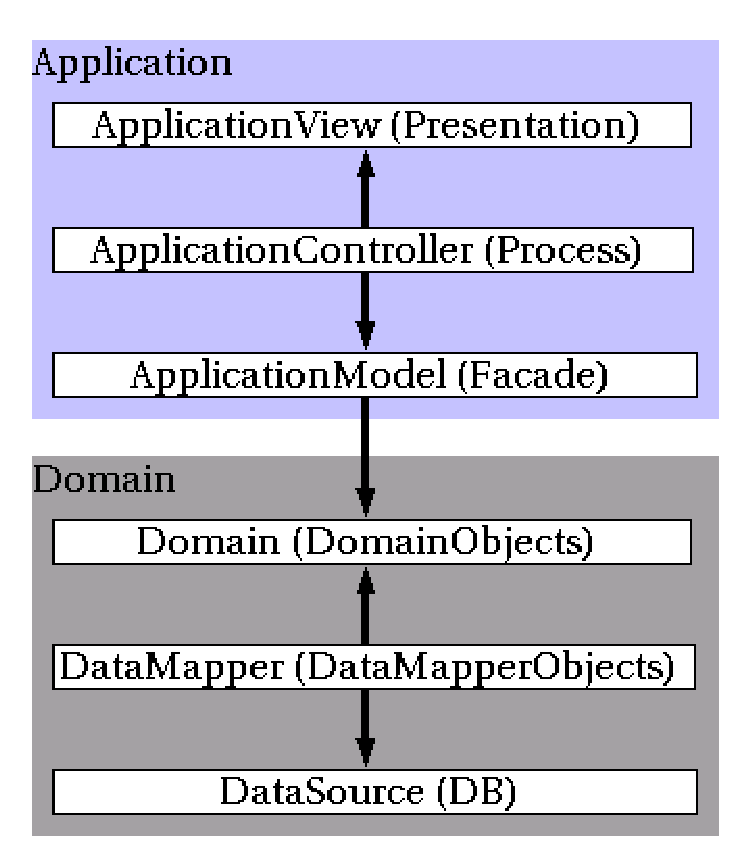
\includegraphics[scale=0.3]{vector/layered_architecture.eps}
        \caption{Layered Architecture}
        \label{layered_architecture_figure}
    \end{center}
\end{figure}

A state-of-the-art software system consists of a layered architecture similar to the
one shown in figure \ref{layered_architecture_figure}. The startable \emph{Controller}
process creates the whole application tree, to which belong the \emph{View} (as
user interface), the \emph{Model} (providing data to the view and as facade to
remote servers) and the \emph{Domain} with its database \emph{Mapper} layer.\\
It is not difficult to figure out where the basic patterns of section \ref{basic_patterns_heading}
fit in here (figure \ref{layered_architecture_with_basic_patterns_figure}):
The \emph{Model View Controller} pattern determines the classes to interact with
a human user via the \emph{View} (sometimes called \emph{Presentation Layer});
the \emph{Data Mapper} pattern provides necessary classes and an \emph{Entity
Relationship Model} (ERM) to connect to a persistence medium such as a database;
the \emph{Data Transfer Object} (DTO) pattern, finally, serves as means of
communication with remote servers.

\begin{figure}[ht]
    \begin{center}
        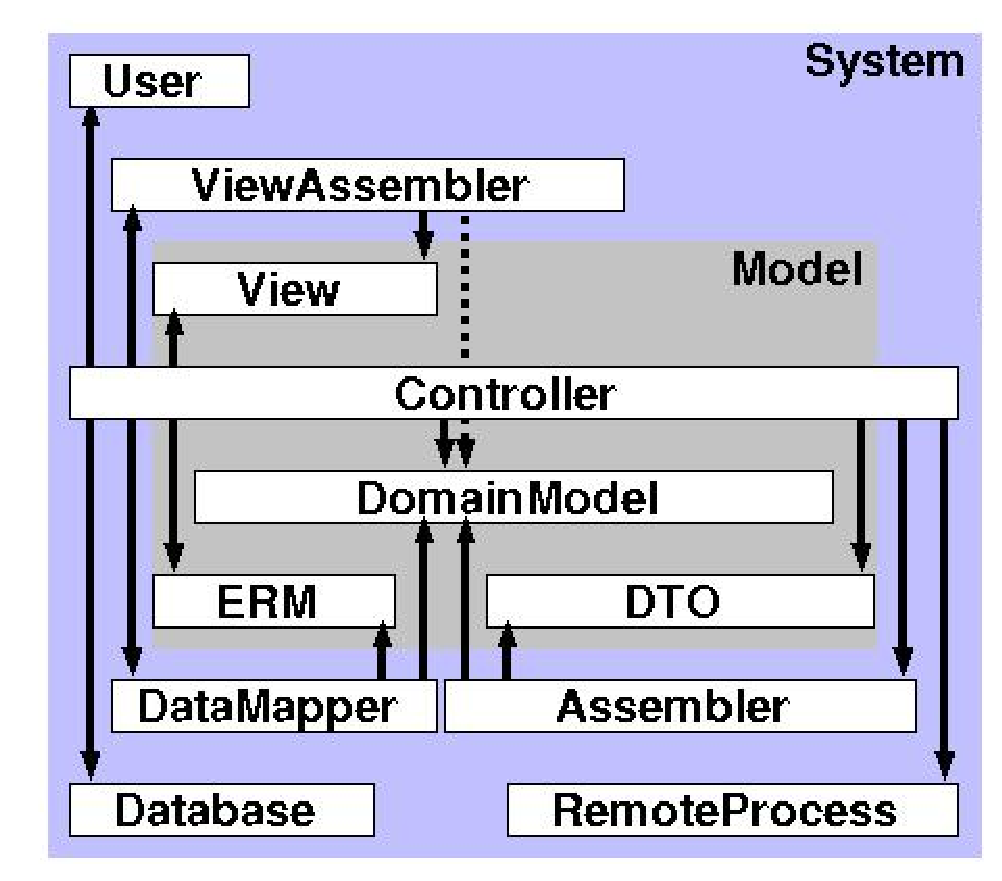
\includegraphics[scale=0.3]{vector/layered_architecture_with_basic_patterns.eps}
        \caption{Layered Architecture with Basic Patterns}
        \label{layered_architecture_with_basic_patterns_figure}
    \end{center}
\end{figure}

For all three kinds of communication, there is a:
\begin{itemize}
    \item[-] System (HumanUser, DataBase, RemoteServer)
    \item[-] Model (View, ERM, DTO)
    \item[-] Translator (ViewAssembler, Mapper, DTOAssembler)
\end{itemize}

Realizing this, it is easy to create ontological layers by adding one common
parent class for systems, models and translators each, which leads to a much
clearer architecture (figure \ref{layered_architecture_with_merged_patterns_figure}).
The common properties of all sub classes are merged into their corresponding super
class.

\begin{figure}[ht]
    \begin{center}
        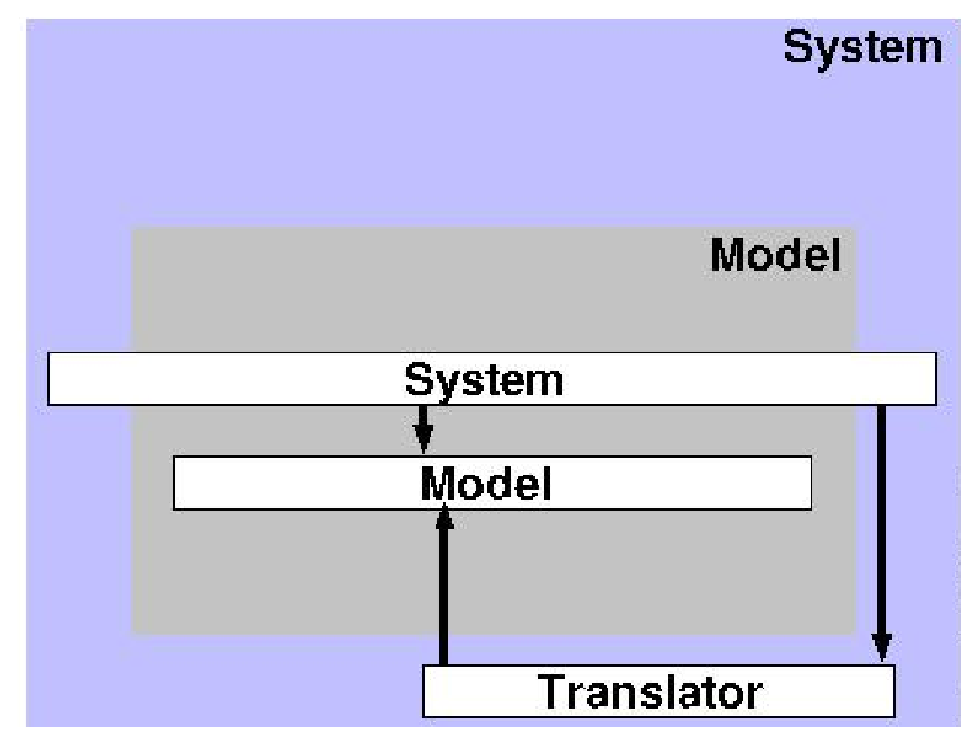
\includegraphics[scale=0.3]{vector/layered_architecture_with_merged_patterns.eps}
        \caption{Layered Architecture with merged Patterns}
        \label{layered_architecture_with_merged_patterns_figure}
    \end{center}
\end{figure}

